\section{Question access when decoding fixed physiological states}

\label{app:question-decoder}

The physiological pilot leaves open whether the readout can retrieve the location of the queried object from a shared neural state. We isolate this interface by holding the initial encoder and physiological core fixed and varying whether the decoder receives the question identity. The frozen language model receives the natural-language question in both conditions.

\paragraph{Matched comparison.}

Both decoders map the same cached 768-dimensional final voltage and synaptic-state vector to eight soft tokens. One decoder receives three zero channels; the other receives a one-hot identity for the queried object (key, coin, or ring). This identity contains no location label. Layer sizes, initialization, minibatch order, and optimizer settings match within each seed. Query-column weights start at zero, giving exactly equal initial prefixes. The state-only decoder has 768 inactive query-column coefficients, so nominal parameter counts match while the additional channel changes which coefficients can learn. Normalization uses training-state means and sample standard deviations, floored at 0.01, with standardized values clipped to $[-10,10]$.

The comparison uses 1,728 training, 288 validation, and 288 test examples. Each of three initializations receives 1,000 updates with batch size 16, Adam learning rate 0.001, and full-validation evaluation every 250 updates. Validation first-answer-token NLL selects the checkpoint independently for each arm; selected checkpoints range from update 500 to 1000. Both checkpoint choices within each seed are fixed before that seed's test evaluation. At evaluation, the language model receives only the decoded state and question. History sentences supply the legitimate event facts to the frozen physiological encoder; history text is never supplied to the primary language-model arms. Training uses answer-token supervision, and evaluation targets are kept separate from feature export and prediction.

\begin{table}[t]
\centering\small
\setlength{\tabcolsep}{3.5pt}
\caption{Question access at the decoder, with the encoder and physiological states held fixed. Values are mean $\pm$ sample standard deviation over three initializations; this is not a confidence interval. Accuracy columns are percentages on the same 288 examples. Earlier/latest identify which object's location is queried; Both requires correct answers to both questions about one history. NLL is the first-answer-token negative log-likelihood in nats. Invalid generated answers count as errors. Chance accuracy is 25\%. The test split was used by the previous pilot and is reused here for exploration.}
\label{tab:question-decoder}
\begin{tabular}{@{}llrrrrr@{}}
\toprule
Decoder & State & Overall & Earlier & Latest & Both & NLL $\downarrow$ \\
\midrule
State only & Intact & 30.0 $\pm$ 3.4 & 36.8 $\pm$ 6.2 & 23.1 $\pm$ 1.6 & 9.0 $\pm$ 0.0 & 1.50 $\pm$ 0.17 \\
State only & Train mean & 17.1 $\pm$ 14.9 & 16.7 $\pm$ 14.4 & 17.6 $\pm$ 15.3 & 4.4 $\pm$ 3.8 & 5.25 $\pm$ 5.54 \\
State only & Paired swap & 14.1 $\pm$ 3.3 & 5.1 $\pm$ 7.1 & 23.1 $\pm$ 1.6 & 0.7 $\pm$ 1.2 & 1.94 $\pm$ 0.04 \\
\midrule
State + question & Intact & 28.7 $\pm$ 2.9 & 31.5 $\pm$ 4.1 & 25.9 $\pm$ 1.7 & 8.3 $\pm$ 2.5 & 1.50 $\pm$ 0.05 \\
State + question & Train mean & 22.7 $\pm$ 4.2 & 22.2 $\pm$ 4.8 & 23.1 $\pm$ 4.2 & 5.8 $\pm$ 2.1 & 2.07 $\pm$ 0.83 \\
State + question & Paired swap & 16.8 $\pm$ 2.4 & 7.6 $\pm$ 3.2 & 25.9 $\pm$ 1.7 & 2.3 $\pm$ 0.8 & 1.86 $\pm$ 0.10 \\
\bottomrule
\end{tabular}
\end{table}


\paragraph{Observed decoding performance.}

The question-conditioned decoder obtains 28.70\% mean strict generated-answer accuracy, compared with 29.98\% for the state-only decoder. Their paired difference is -1.27 percentage points, with a whole-group bootstrap interval of $[-5.44, 2.89]$ and a seed-and-group interval of $[-7.87, 4.86]$. The individual seed differences are $+0.00$, $-5.56$, $+1.74$ percentage points. Mean answer-token NLL is 1.501 versus 1.501 nats; the conditioned-minus-state-only difference is less than 0.001 nats in magnitude. Table~\ref{tab:question-decoder-contrasts} also reports joint-answer and paired-history criteria.

\paragraph{Dependence on the supplied state.}

We replace every state with the training-state mean, and separately substitute the state from the opposite-order history while keeping the queried object unchanged. Replacing a state with its training mean removes history-specific variation but can also move the decoder away from the distribution of states seen during training. The paired swap uses an actual history state and preserves the multiset of events while changing which of the target object's moves occurred last; the distractor object's answer remains unchanged. Control outputs are scored against each recipient's original answer.

For the state-only decoder, intact, mean-state, and swapped-state overall accuracies are 29.98\%, 17.13\%, and 14.12\%, respectively. On earlier-object questions, swapping changes accuracy from 36.81\% to 5.09\%; the intact-minus-swapped difference has group interval $[26.16, 37.50]$ percentage points.

For the question-conditioned decoder, intact, mean-state, and swapped-state overall accuracies are 28.70\%, 22.69\%, and 16.78\%, respectively. On earlier-object questions, swapping changes accuracy from 31.48\% to 7.64\%; the intact-minus-swapped difference has group interval $[18.29, 29.63]$ percentage points.

Valid-answer fractions on intact states are 99.65\% and 99.77\% for the state-only and question-conditioned decoders. With the training-mean state these become 66.67\% and 88.89\%. All mean-state outputs are invalid for seed 715, state-only decoder. The mean-state accuracy decrease therefore mixes changed input information with response-format failures under an altered state distribution; it is not an isolated estimate of the causal contribution of history information.

\begin{table}[t]
\centering\small
\caption{Paired differences, question-conditioned minus state-only decoder. Positive accuracy differences and negative NLL differences favor conditioning. Intervals use 10,000 bootstrap samples of the 72 whole counterfactual groups; the final column additionally resamples the three initialization indices. These intervals describe this exploratory reused split and three seeds, not population-level architecture superiority. Both paired histories correct requires correct answers for the same queried object under both event orders.}
\label{tab:question-decoder-contrasts}
\begin{tabular}{@{}lrrr@{}}
\toprule
Metric & Mean difference & Group interval & Seed + group interval \\
\midrule
Overall accuracy (pp) & -1.27 & $[-5.44, 2.89]$ & $[-7.87, 4.86]$ \\
Earlier-object accuracy (pp) & -5.32 & $[-12.04, 1.16]$ & $[-14.81, 3.94]$ \\
Latest-object accuracy (pp) & +2.78 & $[-2.55, 8.10]$ & $[-5.09, 10.42]$ \\
Both questions correct (pp) & -0.69 & $[-4.17, 2.78]$ & $[-5.56, 4.63]$ \\
Both paired histories correct (pp) & -4.40 & $[-8.56, -0.23]$ & $[-9.72, 0.93]$ \\
Answer-token NLL (nats) & 0.00 & $[-0.07, 0.07]$ & $[-0.17, 0.16]$ \\
\bottomrule
\end{tabular}
\end{table}


\paragraph{Post-hoc numerical reference.}

After inspecting the first seed's language-model test result, we applied the already-used ridge-regression recipe with fixed $\lambda=10$, one four-score head per queried object, and its original Torch float32 train-only normalization. No hyperparameters were tuned or models selected using the new test results. The reference exactly reproduces the previous validation predictions (55.56\% accuracy). On the shared test states it obtains 56.60\% accuracy: 92.36\% for the earlier object and 20.83\% for the latest object. Test accuracy is 25.00\% with the training-mean state and 11.11\% with the paired-swapped state. This is a post-hoc numerical classifier reference, not language generation, an exposure-matched architecture comparison, or a ceiling on recoverable information. Its four-score cross-entropy is not compared with the language model's full-vocabulary token NLL.

\paragraph{Scope.}

This experiment measures retrieval through a particular decoder under a fixed physiological representation. It does not train the connectome or compare biological connectivity with a rewired or conventional recurrent core. The same test split was already evaluated in the preceding pilot; the present analysis is exploratory reuse rather than fresh confirmation. Bootstrap intervals preserve whole counterfactual groups, but three initialization seeds provide only limited evidence about optimization variability. A decoder effect therefore cannot establish a new memory mechanism or a general advantage of connectome-based architectures.

\begin{figure}[t]

\centering

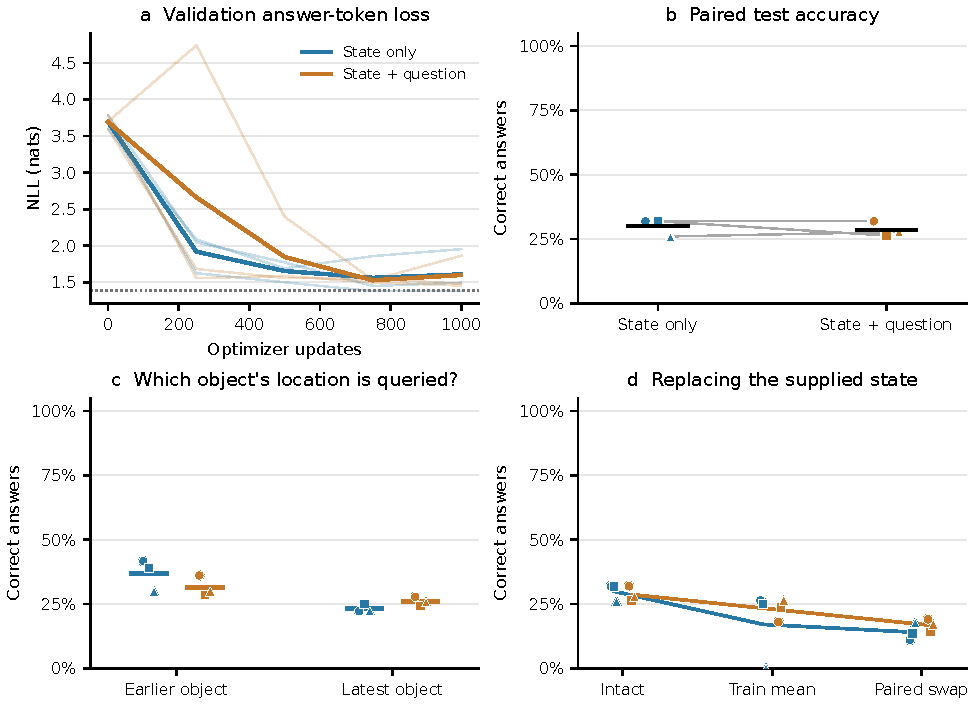
\includegraphics[width=\linewidth]{figures/question_decoder_results.pdf}

\caption{Decoding the same fixed physiological states with and without question identity at the decoder. (a) Full-validation first-answer-token NLL; thin curves show three initializations and thick curves their mean. The dotted line marks $\log 4$, a uniform distribution over four color tokens. (b) Strict test accuracy; connected points pair initialization seeds, and black marks show means. (c) Accuracy by the queried object's position in the history, with individual seeds overlaid. (d) Overall accuracy under intact, training-mean, and paired-swapped states. Accuracy panels use a common 0--100\% scale; dotted lines mark 25\%. The plot retains all three seeds and both decoder arms.}

\label{fig:question-decoder}

\end{figure}
